\documentclass[oneside]{scrreprt}

\usepackage[utf8]{inputenc}

\usepackage[backend=biber,style=chem-biochem]{biblatex}
\usepackage{blindtext}
\usepackage{graphicx}
\usepackage{abstract}
\usepackage[headsepline]{scrlayer-scrpage}
\usepackage{listings}
\usepackage[hidelinks,bookmarks,urlcolor=blue]{hyperref}
\usepackage{mathtools}
%\usepackage{ftnright}
\pagestyle{scrheadings}
\graphicspath{ {./pics/} }
\usepackage{xcolor}
\usepackage{soul}
\usepackage{url}
\usepackage{svg}

\definecolor{Light}{gray}{.90}
\sethlcolor{Light}



\newcommand{\code}[1]{\texttt{\hl{#1}}}

\addbibresource{BSc_Thesis_Bibliography.bib}
\title{Relative binding free energy calculations of restrained systems in the 'common-core serial-atom-insertion' framework}
\author{Supervised by: Univ-Prof. Dr. Stefan Boresch\\Submitted by: \hspace{26mm}Alexander Grasser}
\date{June 2022}
\publishers{Department of Computational Biological Chemistry\\University of Vienna\\
\includegraphics[width=5cm]{Uni_Logo_2016.jpg} }
\subject{Thesis for the title Bachelor of Science in Chemistry}

\automark[chapter]{chapter}
\ihead{Bachelor's Thesis}
\chead{}

\ohead{\headmark}


\RedeclareSectionCommand[pagestyle=scrheadings,beforeskip=0pt]{chapter}






\begin{document}

\begin{titlepage}

\maketitle{}
\end{titlepage}
\section*{Abstract}
    
    For Protein-Ligand affinity at binding sites, the relative (and absolute) binding free energy is arguably the most important indicator. Traditionally, calculating these energies is done using comprehensive, GPU-assisted "soft-core" modelling. The 'common-core serial-atom-insertion' framework \texttt{Transformato} instead allows to efficiently divide the problem into sequential fragments solvable by traditional MD calculations. However, issues arise when ligands leave the binding site during simulation. This has been addressed by adding restraints to the system.
\vspace{\fill}
\section*{Notes}
\noindent\begin{minipage}{0.7\textwidth}
The data underlying this thesis may be accessed at github under \url{https://github.com/agrass15268/AuxiliaryRestraintsTransformato/tree/data} or with the QR - Code to the right.
\end{minipage}
\hspace{0.1\textwidth}
\begin{minipage}{0.2\textwidth}
\includesvg[height=2cm]{qrcode}
\end{minipage}
\newpage

\begingroup
\let\clearpage\relax
\renewcommand\contentsname{Table of Contents}
\tableofcontents
\addtocontents{toc}{~\hfill\textbf{Page}\par}
\endgroup
\renewcommand{\thefootnote}{\Roman{footnote}}
\chapter{Introduction}
Almost since the inception of computer-assisted molecular modelling, a significant focus has been on the interaction of pharmaceutically active biomolecules. Designing and testing lead compounds to catalyze or inhibit biochemical processes is a major focus of research and development efforts, and a comparatively easy to access parameter with nevertheless good predictive capabilities has long been the relative binding free energy difference. However, traditional molecular dynamics (MD) modelling efforts face the so-called van-der-Waals endpoint problem when trying to do either alchemical or physical energy simulations. Circumventing these problems requires the use of soft-core-potentials, which significantly increases computing costs and does not fully solve these problems. Recently, the package \texttt{Transformato} was introduced by Karwounopoulos, Wieder, Braunsfeld and Boresch\supercite{Karwou2022Jun,braunsfeldImplementationTestingCHARMM,Wieder2022Jun}, implementing a novel approach bypassing these problems. Being a python pacakge, \texttt{Transformato} is easy to install, use, and modify to adapt to system-specfific challenges or support different MD engines. Instead of full alchemical transformations of one compound into the other, it instead relies on computing a \emph{common core} (CC) between the two physical endpoints. Summing up the energy differences between the CC and the endstates allows calculation. 
\chapter{Theory}

\section{Theoretical Background}



\begin{figure}[h]
\centering
 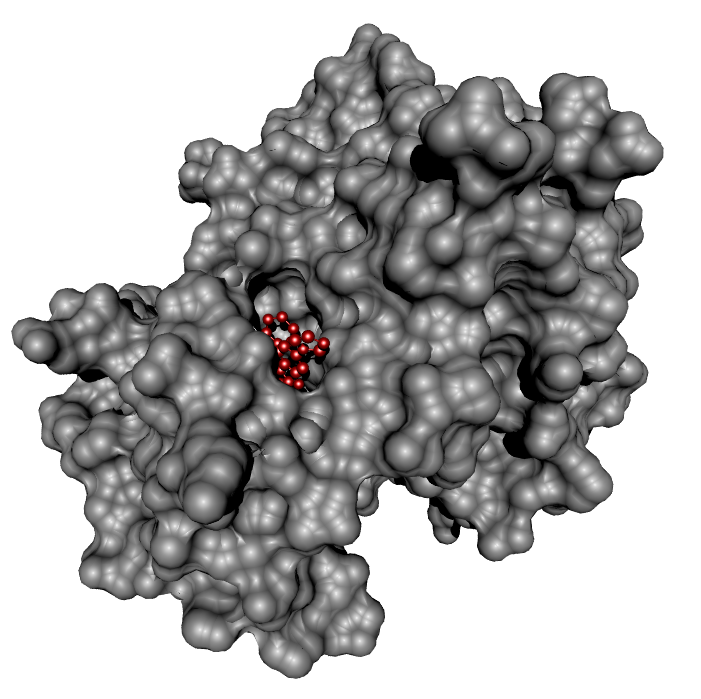
\includegraphics[height=4cm]{2oj9_render_complex.png} 

\caption{VMD Render of 2OJ9. Highlighted in red: The ligand BMI}
\label{fig:vmdrender}
\end{figure}
Above, in Figure \Ref{fig:vmdrender} you can see the effects rendering a molecule has.


\subsection{Basics of Molecular Dynamics Modeling}

Since the discovery of cells, the inner workings of biological systems have always been a mystery science has raced to solve. While of course physical methods have allowed some degree of monitoring biochemical processes, these have significant limits - most glaringly being limited to actually physically-present structures. With Molecular Dynamics (MD) on the other hand, it is entirely possible to observe molecular interactions as they would happen in reality - at the leisure and convenience of the observer, with an unmatched resolution and clarity, and without the need to synthesize a single atom - the so-called \emph{ab silico} - approach.

In general, MD aims to simulate the movement of atoms in a molecular system over time, governed by the physical interactions present in the molecule \supercite{Hollingsworth2018Sep}. Unlike quantum chemistry simulations, which try to calculate interactions using various approximations or even solutions of the Schrödinger equation, MD simulations have no pretensions of being an exact science. Instead, forces are approximated by what are essentially the mechanical principles of Newton: Atoms are perfect spheres, with mass and charges, and all their interactions are defined by a set of forces governing the interactions of specific types of atoms. As such, the kinetic energy of an MD system is simply the kinetic energy of atom masses at speed, and their potential energy defined by the potentials governing their interactions.

For almost all force fields, forces in MD simulations may be divided into two parts - \emph{bonded} and \emph{nonbonded} interactions. These are often used synonymously with \emph{intermolecular} and \emph{intramolecular} forces, but are far from the same - it is quite possible, and especially in biological systems the rule more than the exception, that nonbonded interactions contribute a significant part to the intramolecular structure.

Bonded forces are generally given explicitly for each atom types. They are:
\begin{itemize}
    \item Bonds (across two atoms)
    \item Angles (the angle across three atoms)
    \item Dihedrals (the angle across four atoms)
    \item Impropers (the angle of a fourth atom being out-of-plane with the other three)
\end{itemize}

All of which are defined in \emph{parameter files}, which contain the force parameters for each of these.

\begin{figure}
\tiny
\begin{verbatim}
BONDS
CG1N1  CG2R51  375.00     1.4220 ! DCG, yxu, RNA
CG1N1  CG2R61  345.00     1.4350 ! 3CYP, 3-Cyanopyridine (PYRIDINE pyr-CN) (MP2 by kevo)
CG1N1  CG321   400.00     1.4700 ! CYU, from CG1N1 CG331, yxu, RNA
CG1N1  CG331   400.00     1.4700 ! ACN, acetonitrile, kevo
CG1N1  NG1T1  1053.00     1.1800 ! ACN, acetonitrile; 3CYP, 3-Cyanopyridine (PYRIDINE pyr-CN) (MP2 by kevo)
CG1N1  SG311   328.79     1.7011 ! XCN, by ac_aa            

ANGLES
CG2R51 CG1N1  NG1T1    40.00    180.00 ! DCG, yxu, RNA
CG2R61 CG1N1  NG1T1    40.00    180.00 ! 3CYP, 3-Cyanopyridine (PYRIDINE pyr-CN), yin
CG321  CG1N1  NG1T1    21.20    180.00 ! CYU, from CG331 CG1N1 NG1T1, yxu, RNA
CG331  CG1N1  NG1T1    21.20    180.00 ! ACN, acetonitrile, kevo
NG1T1  CG1N1  SG311    40.70    179.93 ! XCN, by ac_aa                
CG1T1  CG1T1  CG331    19.00    180.00 ! 2BTY, 2-butyne, kevo
CG1T2  CG1T1  CG2D1    11.00    180.00 ! BEYN, pchat
CG1T2  CG1T1  CG321    11.00    180.00 ! BUTY , PNTY, HPTY, HXYN,OCTY , pchat

DIHEDRALS
NG1T1  CG1N1  CG2R61 CG2R61  0.0100 2    0.00 ! CNP2, by ac_aa
NG1T1  CG1N1  SG311  CG321   0.0060 1    0.00 ! XCN, by ac_aa
CG2R53 CG251O CG25C1 CG2R53     6.4000  2   180.00 ! OIRD, oxindol-3-ylidene rhodanine, kevo & xxwy
CG2R53 CG251O CG25C1 CG2RC0     6.4000  2   180.00 ! OIRD, oxindol-3-ylidene rhodanine, kevo & xxwy
NG2R53 CG251O CG25C1 CG2R53     3.4000  2   180.00 ! OIHY, 5-(oxindol-3-ylidene)hydantoin, complete ring system, xxwy
NG2R53 CG251O CG25C1 CG2RC0     3.4000  2   180.00 ! OIHY, 5-(oxindol-3-ylidene)hydantoin, complete ring system, xxwy
SG311  CG251O CG25C1 CG2R53     6.4000  2   180.00 ! OIRD, oxindol-3-ylidene rhodanine, kevo & xxwy
SG311  CG251O CG25C1 CG2RC0     6.4000  2   180.00 ! OIRD, oxindol-3-ylidene rhodanine, kevo & xxwy

IMPROPERS
CG2D1  CG331  NG2D1  HGA4      25.00  0     0.00 ! SCH1, xxwy
CG2D1  CG331  NG2P1  HGR52     18.00  0     0.00 ! SCH2, xxwy
CG2D1O CG2DC1 CG2O1  NG2S1   28.3025 0    0.00 ! DYAP, by ac_aa              
CG2D1O CG331  NG2D1  SG311   18.8025 0    0.00 ! FZN, by ac_aa
\end{verbatim}
   \caption{Excerpt from a parameter file created by CGenFF with a few definitions from bonds, angles dihedrals and impropers each.}
    \label{fig:parmfile}
\end{figure}

As apparent in figure \ref{fig:parmfile}, force-field parameter files are structured very simply: The first few columns define the "atom types" for which a given set of parameters is valid. The others define the numeric value of the various parameters for the potential; for simple bonds for example the first value denotes the force constant, and the second the equilibrium distance. These values are inserted into a harmonic potential and then used to calculate the force. 


In a MD system, the combined potential energy is simply the sum of bonded and nonbonded potential energy terms, both of which are dependent on the relative positions $(\Vec{r})$ of the atoms:


\begin{equation}
    \sum U (\Vec{r}) = \sum U_{bonded} (\Vec{r}) + \sum U_{nonbonded} (\Vec{r})
\end{equation}

The sum for bonded potentials is the sum of the individual potentials:

\begin{equation}
    \sum U_{bonded} (\Vec{r})=\sum U_{bonds} (\Vec{r}) + \sum U_{angle} (\Vec{r}) + \sum U_{torsion} (\Vec{r}) +\sum U_{improper} (\Vec{r})
\end{equation}

Whereas the nonbonded potentials \emph{generally} consist of electrostatic (Morse) and VdW (Lennard-Jones) Potentials.

\begin{equation}
    \sum U_{nonbonded} (\Vec{r})=\sum U_{electrostatics} (\Vec{r}) + \sum U_{Lennard-Jones} (\Vec{r})
\end{equation}




\subsection{Relative and absolute binding free energies}

Calculating the free energies however, is a somewhat more problematic undertaking. For our purposes, we need to differentiate two types of free energy:
\begin{itemize}
    \item \emph{solvation} free energies, which describe the energy difference between solvated and unsolvated compunds;
    \item \emph{binding} free energies, which describe the energy difference between a ligand bound to a complex, and an unbound one
\end{itemize}
They are however calculated using similar principles - by exploiting thermodynamic cycles.

\subsection{Soft-core potentials and the van-der-Waals endpoint problem}
In a standard MD simulation, the Lennard - Jones interaction $U_{LJ}$ is given by formula \ref{eq:ljstandard}.
\begin{equation}
U_{LJ}(r,\lambda)=(1-\lambda)(\frac{A}{r^{12}} - \frac{B}{r^6})
\label{eq:ljstandard}
\end{equation}
This usually works rather well -  the shape of the potential ensures that no two LJ particles inhabit the same spot. However, free energy calculations for the reasons discussed above, usually require the presence of \textit{dummy atoms} - which obviously do not have Lennard - Jones interactions. It's rather obvious, where problems may now occur -  as there are not LJ interactions, atoms may move freely into each other. This may not seem like such a significant problem - but forces still need to be calculated. Should particles manage to inhabit the exact same position, this would result in a division by zero - problematic, but most modern MD software can handle this. 

Both more problematic and more common, however, is the case that two particles get very close to each other. In this case, the derivation $\langle \frac{\delta U}{\delta\lambda} \rangle$ may diverge, causing the entire simulation to become unstable. This is known as the \textit{van-der-Waals endpoint problem} (or \textit{-catastrophe}, for the more dramatically inclined).

To avoid this problem, soft-core potentials were introduced as shown in Equation \ref{eq:ljsoftcore}\supercite{Beutler1994Jun}:
\begin{equation}
U_{LJ}^{SC}(r,\lambda)=(1-\lambda)(\frac{A}{(r^2 +\lambda \delta)^6 }-\frac{B}{(r^6 +\lambda \delta)^3})
\label{eq:ljsoftcore}
\end{equation}
These mostly solve the problem, as there can now be no division by zero and the fractions remain finite in all circumstances. They are, however, computationally expensive and complicate free energy calculations using mBAR or TI\supercite{Li2020Aug}. It is important to note that \texttt{Transformato} for this reason does \textbf{not} use soft-core potentials.


\section{The common-core serial-atom-insertion framework {\texttt{Transformato}}}
To address these problems, the common-core serial-atom-insertion framework was conceptualised and implemented in \texttt{Transformato}. \texttt{Transformato} is engine-agnostic - its outputs being designed to be computable with any of the widely-used Molecular Dynamics engines (openMM, CHARMM, AMBER, GROMACS etc.), though preprovided simulation scripts are currently only available for CHARMM and openMM.


\subsection{Theoretical Principles}
\subsection{Theoretical consideration for Restraints in \texttt{Transformato}}
\subsection{Usage}
Installing \texttt{Transformato} is fairly straightforward: it requires a working installation of \texttt{conda} and \texttt{python}. Using \texttt{git clone}, download the package from the repository\footnote{\url{https://github.com/JohannesKarwou/Transformato}} and run \texttt{python setup.py install}. This will install a conda environment called \texttt{fep} consisting of \texttt{Transformato} and all its dependencies. Activate the environment and you're done.

To calculate free energies, retrieve a PDB containing your ligand-protein complex for both endpoints. For each, solvate once the complex including the ligand and once just the ligand using e.g. CHARMM-GUI's Solvation Builder\footnote{\url{https://www.charmm-gui.org/}}. Take the output folders, equillibrate them and name the 'complex' and 'waterbox', respectively. You will then need to create a config.yaml file containing the names of your structures and parameters you want your simulation to have - any restraints you wish to apply must also be defined here. The simplest case for specifying restraints is simply done by adding the keyword \code{restraints: auto} to the \emph{simulation} part of the configuration file. This restrains the entire ligand backbone via its center of mass to the center of mass of the protein backbone. Inside the code, this is referred to as \texttt{simple} mode. Another possibility is the generation of restraints on the extremities of the ligand using the \code{extremities=[int]} keyword. This algorithmically selects those carbon atoms furthest from the center of mass (and each other), and restrains these and their surroundings to the protein, thus cutting down on rotational freedom. The downside of this is that it requires some prior knowledge of the ligand's shape - not usually a problem, but potentially in large-scale applications. Of course, this also reduces sampling volume even further than the simple restraint. Lastly, it is also possible to manually define restraints in addition to - or instead of - the automatic ones, using the keyword \code{restraints: manual} and defining manual restraints below. This allows full use of the MDAnalysis\supercite{agrawal2011,oliver_beckstein-proc-scipy-2016} selection syntax, limited only by the common core on the ligand.

\begin{figure}\small

\begin{verbatim}
Free energy to common core: 12.02382 [kT] with uncertanty: 0.5843413703 [kT].
Free energy difference: 12.02382 +- 0.584341 [kT]
Both states are considered
\end{verbatim}
\label{fig:anaoutput}
\caption{Typical output of analysis.py}
\end{figure}

To actually create the simulation runs, you will need a modified 'submit.ipynb'. These files sequentially load the .yaml config and the structure topologies, then propose a common core. After this point, you may add (or remove) atoms from the common core. Afterwards, \texttt{Transformato} will propose a mutation route. If it looks satisfactory, it will then create a number of folders containing intermediate states, each a self-contained simulation. Simulate these (as this is the most computationally intensive step, it is highly recommended to use a cluster for this step) and run the analytics script (a cluster is also recommended here). At the end, you should receive output similar to Figure \ref{fig:anaoutput}. Please note that the energy difference to the common core is usually only one leg of the journey; unless one of the endstates is identical to the common core, you will need to add the values for both to get the actual relative free energy. 

A significantly more extensive documentation of \texttt{Transformato}'s abilities and features is available through the github repositories wiki at \url{https://github.com/JohannesKarwou/Transformato/wiki}, along with sample input and data files.


\chapter{Methods}
\section{Implementation of restraints into \texttt{Transformato}}

The process of applying restraints was divided into four parts:

\begin{enumerate}
    \item Processing user input: the general demand for restraints, and parameters for these restraints
    \item Finding suitable binding sites and generating the atom selections for the restraints
    \item Generating an openMM Force object
    \item Applying this Force to the actual simulation

\end{enumerate}

These processes were complicated by the fact that the script that generates the intermediate states for processing (and thus have access to user input) are separate from those that do the actual simulations (which need to be independent to be able to run on distributed computing networks).



 As much code as possible was exiled into a seperate module file called \code{restraints.py}, with only minimal changes to \code{state.py} and \code{mutate.py} being necessary. 

Currently, restraints are only available as a proof-of-concept for openMM. OpenMMs \emph{CustomCentroidBondForce} was chosen as basis for all restraints. To facilitate analysis of Ligand and Protein structures, MDAnalysis\supercite{agrawal2011,oliver_beckstein-proc-scipy-2016} was used.

\subsection{Processing user input}
To leverage the existing codebase as well as keeping with the established desing principles of \texttt{Transformato}, additional user input was restricted to the configuration \texttt{.yaml} already required; and to ensure both backwards compatibility and prevent accidental use of restraints all commands to use restraints are purely optional. If a user is unaware of the possibility of restraints, they will not run into danger of accidentally using them. Further, there is no additional workflow in the users's submit script - all of it is done during \code{utils.py::load\_config\_yaml()} automatically.

Due to the structure of the existing code, no changes to \code{utils.py} were necessary - all relevant information was available for further processing immediately.
\subsection{Finding suitable restraints}

\subsection{Generating an openMM Force object}

\subsection{Applying the Force to the actual simulation}
\section{RBFE calculations}
All inputs were generated using CHARMM-GUI\supercite{Jo2008Aug}, and used the CHARMM36m forcefield\supercite{Huang2017Jan}. For easier handling and allowing larger timesteps, CHARMM-GUI's facility for hydrogen mass repartitioning\supercite{Gao2021Feb} was used unless noted. Equillibration was done using the openMM - Inputs provided by CHARMM-GUI\supercite{Brooks2009Jul,Lee2016Jan}. To modify the ligand, CHARMM-GUI's ligand designer\supercite{Guterres2021Nov} was used alongside the commercial program Maestro\supercite{maestro}. The simulations themselves were carried out using openMM 7.5\supercite{Eastman2017Jul}


\subsection{2OJ9 - Tautomer A with modified BMI}
\subsection{2OJ9 - Tautomer B with modified BMI}
\subsection{Vim2 with ZN148 and ZN223}
Vim2 is a Carbapenem-Hydrolyzing Metallo-$\beta$-Lactamase, responsible for a subtype of bacterial drug resistance.\supercite{Poirel2000Apr}. ZN148 and ZN223 are specific zinc ligands first presented by Samuelsen et al.\supercite{Samuelsen2020Jun}. These ligands are designed to inhibit Vim2 activity and suppress its drug-resistant activity, thus providing a treatment vectory for strains containing it. 

To prepare the structures for use in transformato, protonation states were determined by use of ProToss\supercite{Lippert2009Dec,Bietz2014Dec} and manual observation, after which ligand and protein were solvated using CHARMM-GUI's solvation builder, including patching of the C-Terminus. As certain binding modes require the presence of an OH$^-$ group nearby, but CHARMM-GUI's solvation builder is unable to process the system with it, a roundabout way was chosen were a seperate .crd file for the OH group was created and patched in after solvation using \texttt{macha}\supercite{twotoneblue2022May}. As this also complicated HMR, Hydrogen Mass Repartitioning was accomplished using \texttt{parmed}\supercite{Shirts2016Sep}. Afterwards, use in \texttt{Transformato} continued as normal.



\chapter{Results}

\section{Application of restraints to classical MD simulations}

\section{Application of restraints to \texttt{Transformato} RBFE calculations}
\subsection{2OJ9: Tautomer A, BMI 24 to 25}
\begin{table}\small
\begin{center}
    \begin{tabular}{l|r|l|r|r}
        Restraints & k - value & scaling & Average [kT] & SD [kT]   \\
        \hline
        Extremities & 100 & no  & -1.15 & 2.15                                   \\
        Extremities & 100 & yes & 0.11  & 1.95                                   \\
        Simple      & 100 & no  & 0.09  & 1.22                                   \\
        Simple      & 100 & yes & -0.97 & 0.41  \\
        Extremities & 10  & no  & -1.87 & 0.04   \\
        Extremities & 10  & yes & -1.30 & 1.69                                   \\
        Simple      & 10  & no  & 0.30  & 1.45                                   \\
        Simple      & 10  & yes & -0.74 & 0.77   \\
        Extremities & 3   & no  & -0.35 & 1.73                                   \\
        Extremities & 3   & yes & 0.27  & 1.00                                   \\
        Simple      & 3   & no  & -1.82 & 0.50   \\
        Simple      & 3   & yes & -2.05 & 2.61                                   \\
        Extremities & 400 & no  & 1.11  & 2.89                                   \\
        Extremities & 400 & yes & 5.39  & 1.31                                   \\
        None        & N/A & no  & -1.07 & 1.08                                  
    \end{tabular}
\end{center}
\caption{2OJ9 Tautomer A, $\Delta\Delta G_{bind}L_{24}\xrightarrow{} L_{25}$. Simulation Time: 1.25 ns, Step Time: 1fs, 3 Replicates}
\label{tab:2oj9_taapdb_24to25_shortruns}
\end{table}

\begin{table}\small
\begin{center}
\begin{tabular}{l|l|l|l|l|}
Restraints & k- value & scaling & Average [kT] & SD [kT]\\
\hline
Simple   & 400 & yes & 9.52  & 0.99 \\
Simple & 400 & no  & 9.40  & 1.34 \\
Extremities      & 400 & yes & 8.20  & 1.61 \\
Extremities       & 400 & no  & 10.34 & 0.99 \\
Simple    & 100 & yes & 8.29  & 0.86 \\
Simple  & 100 & no  & 10.10 & 0.21 \\
Extremities         & 100 & yes & 9.36  & 1.45 \\
Extremities       & 100 & no  & 10.24 & 2.33 \\
Simple   & 10  & yes & 8.63  & 0.38 \\
Simple    & 10  & no  & 9.42  & 2.61 \\
Extremities          & 10  & yes & 9.80  & 0.98 \\
Extremities        & 10  & no  & 10.98 & 1.35 \\
Simple     & 3   & yes & 10.00 & 0.41 \\
Simple    & 3   & no  & 9.88  & 1.28 \\
Extremities         & 3   & yes & 9.33  & 1.92 \\
Extremities         & 3   & no  & 9.43  & 1.17 \\
None & N/A & no & 8.77 & 1.85
\end{tabular}
\end{center}
\caption{2OJ9 Tautomer B, $\Delta\Delta G_{bind}L_{24}\xrightarrow{} L_{25}$. Simulation Time: 1.25 ns, Step Time: 1fs, 3 Replicates}
\label{tab:2oj9_tablit_24to25_shortruns}
\end{table}


\chapter{Discussion}

\section{Comparison to experimental results}
\section{Future possibilities }

\listoffigures

\listoftables
\printbibliography[title={References}]%heading=subbibnumbered,
\end{document}